\section{Ohjelmistojen testaaminen ja mobiilisovellusten testaamisen erityispiirteitä}

Tässä luvussa esitellään ohjelmistojen testauksen peruskäsitteitä, testauksen asemaa ohjelmistotuotantoprosessissa, mobiilisovellusten testaamisen erityispiirteitä sekä pohditaan miten testaustyökaluja voi arvioida.

\subsection{Testaamisen peruskäsitteitä}

Testitapaus (test case) on yksittäinen testi, jolle on määritelty syötteet, suoritusehdot ja läpäisykriteerit. Testisarja (test suite) taas on joukko testitapauksia. Testisarja voi myös koostua useasta testisarjasta, jolloin esimerkiksi ohjelman jokaiselle komponentille voi olla oma testisarjansa ja yksi testisarja kattaa sitten kaikki yksittäisten komponenttien testisarjat. \cite[153]{testing}

Yksikkötestauksella (unit testing) tarkoitetaan testejä, joiden kohteena on pienimmät mahdolliset ohjelmakomponentit. Olio-ohjelmoinnissa tämä tarkoittaa useimmiten yksittäistä luokkaa, koska yksittäiset metodit vaikuttavat olion tilaan ja siten metodien toimintaan. \cite[282-286]{testing}. JUnit \cite{junit} on Javan standardi yksikkötestaustyökalu.

Yksikkötestaus on useimmiten valkoinen laatikko -testausta (white box testing / structural testing / glass box testing), jolloin testejä voidaan kirjoittaa ohjelmakoodin perusteella. Testeiltä voidaan vaatia esimerkiksi tiettyä koodikattavuutta, jolloin varmistetaan, että mahdollisimman suuri osa ohjelmakoodista tulee suoritettua testien aikana. \cite[154]{testing}

Toiminnallisessa testauksessa (functional testing) testattavan ohjelman sisäistä rakennetta ei tunneta vaan ollaan kiinnostuttu vain syötteistä ja niitä vastaavista tulosteista. Toiminnallista testausta voidaan kutsua myös musta laatikko -testaukseksi (black box testing) (varmista jostain toisesta lähteestä että nämä ovat oikeasti synonyymi, wikipedian mukaan ei ole vaan functional on black boxin alalaji!) Toiminnallisessa testauksessa ollaan kiinnostuttu ohjelman käyttäjälle näkyvästä toiminnasta ja niitä voidaan tehdä esimerkiksi ohjelman määrittelyn pohjalta. \cite[161-162]{testing}

Mallipohjainen testaus (model based testing) on toiminnallisen testauksen alalaji, jossa testitapaukset luodaan automaattisesti ohjelman spesifikaatiosta tehdystä mallista. Jos ohjelma mallinnetaan formaalilla mallilla, kuten äärellisellä automaatilla tai kieliopilla, voidaan testitapaukset generoida täysin automaattisesti. Semiformaaleilla menetelmillä, kuten luokka- tai oliokaavioilla, mallinnetuista ohjelmista generointi saattaa vaatia manuaalista työtä. \cite[245-250]{testing}

Hyväksyntätestien (acceptance tests) tarkoitus on kertoa, onko ohjelma valmis julkaistavaksi. Hyväksyntätesteissä ei etsitä vikoja ohjelmasta, vaan yritetään varmistaa sen riittävä laatutaso. Hyväksyntätestit ovat usein tilastollisia: niissä mitataan ohjelman luotettavuutta, saavutettavuutta tai häiriötiheyttä. Ongelmana tällaisessa testauksessa on, että vaatii hyvin paljon testiainestoa ennen kuin voidaan olla varmoja ohjelman riittävästä laadusta. Usein hyväksyntätestauksessa käytetään alfa- ja beta-testausta, jolloin ohjelman käyttäjät pääsevät testaamaan ohjelmaa ja raportoimaan sen laadusta. \cite[421-423]{testing}

Mockaus (suomennos?) on tekniikka, joka helpottaa yksikkötestien kirjoittamista. Yksikkötestien ulkoiset riippuvuudet voidaan korvata testeissä kontrolloitavilla mock-olioilla. Tällöin testit ovat vakaampia, koska ulkopuolisten komponenttien muokkaus ei vaikuta testeihin, testin haluttuun lopputulokseen vaikuttava ympäristö on helppo saada haluttuun muotoon. Tällöin testien on helppo testata myös sellaisia olosuhteita, jotka ovat harvinaisia, tai vaikea saada muokattua. Lisäksi mockaamalla voidaan korvata vielä tekemättömät ulkoiset riippuvuudet mock-toteutuksilla. \cite{mocking}

\subsection{Testaaminen osana ohjelmistotuotantoprosessia}

\begin{figure}[htb]
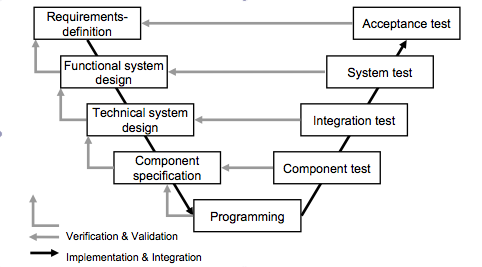
\includegraphics[width=130mm]{v_model.png}
\caption{Testauksen v-malli} \label{v_model}
\end{figure}

Ohjelmistotuotantoprosessia lähestytään yleensä jonkin elämänkaarimallin kautta. Testauksen näkökulmaa edustaa testauksen v-malli, joka on esitetty kuvassa \ref{v_model}. Mallin yleisessä versiossa lähdetään siitä, että jokaista ohjelmistotuotantoprosessin vaihetta vastaa jokin testausvaihe. Näin testaus tehdään ohjelmistotuotantoprosessissa näkyväksi ja yhtä tärkeäksi osaksi kuin itse sovelluksen kehittäminen. Kuvassa v:n vasemmalla haaralla on vesiputousmallin mukaiset ohjelmistotuotantoprosessin vaiheet. Ensimmäisenä vaiheena on vaatimusmäärittely. Tässä vaiheessa määritellään loppukäyttäjän tai asiakkaan tarpeet ja vaatimukset sovellukselle.  Viimeinen vaihe on alimpana oleva sovelluksen ohjelmointi. Oikealla haaralla on testausvaiheet, joissa jokaisessa varmistetaan, että ohjelma täyttää vasemman haaran samalla tasolla olevassa vaiheessa suunnitellut vaatimukset \cite[39-42]{testing_foundations}.

V-mallin alimmalla tasolla on komponentti- eli yksikkötestaus. Siinä testataan ohjelman pienempiä itsenäiseen toimintaan kykeneviä osasia, eli olio-ohjelmoinnin tapauksessa useimmiten luokkia. Android-sovellusten tapauksessa tällä voidaan ajatella yksittäistä Android-komponenttia, esimerkiksi aktiviteettia, tai jopa aktiviteettia pienempiä osia, kuten yksittäistä näkymä-luokkaa tai muuta toimintaa tarjoavaa alikomponenttia. Komponenttitestaus on useimmiten valkoinen laatikko -testausta ja sen suorittaminen vaatii ohjelmointitaitoa. Useimmiten sovelluksen ohjelmoijat suorittavat itse komponenttitestauksen. Komponenttitestauksella pyritään varmistamaan, että komponentti täyttää sen toiminnallisen määritelmän. Komponenttitestejä tehdään usein eri kielille kehitetyillä yksikkötestikehyksillä, kuten Javan JUnitilla. Oikean toiminnallisuuden testaamisen lisäksi on tärkeää testata myös toiminta väärillä syötteillä ja poikkeustilanteissa. Moderni tapa tehdä komponenttitestausta on kirjoittaa testikoodi ennen sovelluskoodia \cite[43-50]{testing_foundations}.

V-mallin seuraavalla tasolla on integraatiotestaus. Siinä vaiheessa oletetaan, että komponenttitestaus on jo tehty ja yksittäisten komponenttien omaan toimintaan liittyvät virheet on löydetty. Integraatiovaiheessa yksittäisten komponentit yhdistetään toisiinsa ja testataan, että niiden yhteistoiminta on oikeanlaista. Tavoitteena on löytää mahdolliset virheet komponenttien rajapinnoista ja komponenttien välisestä yhteistyöstä. Testauksessa voidaan käyttää apuna stubeja (suomennos?) sellaisista komponenteista, jotka eivät vielä ole valmiita \cite[50-52]{testing_foundations}.

V-mallin kolmannella testaustasolla on järjestelmätestaus (system testing). Järjestelmätestauksessa testataan, että täysin integroitu järjestelmä toimii kokonaisuutena kuten pitäisi. Alemmista tasoista poiketen järjestelmätestauksessa näkökulma on järjestelmän tulevan käyttäjän, kun alemmilla tasoilla testaus on luonteeltaan enemmän teknistä. Järjestelmätestauksessa varmistetaan, että järjestelmä kokonaisuudessaan täyttää sille asetetut toiminnalliset ja ei-toiminnalliset vaatimukset. Järjestelmätestauksessa ei tulisi käyttää enää stubeja, vaan järjestelmän kaikki komponentit tulisi asentaa esimerkiksi erilliseen testiympäristöön testausta varten. Itse sovelluksen lisäksi järjestelmätestauksen piiriin kuuluu ohjelmiston dokumentaatio ja konfiguraatio \cite[58-61]{testing_foundations}.

V-mallin viimeinen vaihe on hyväksyntätestaus. Alemmilla tasoilla sovellus on ollut kehittäjän vastuulla, mutta hyväksyntätestauksessa järjestelmä testataan asiakkaan näkökulmasta. Tällöin pyritään varmistamaan, että tuotettu järjestelmä täyttää mahdollisen sopimuksen, että sen käyttäjät hyväksyvät sen käytön sekä mahdollisesti alfa tai beta -testauksen oikeilla järjestelmän loppukäyttäjillä.\cite[62-]{testing_foundations}

Testauksen jokaisessa vaiheessa ollaan kiinnostuneita validoinnista ja verifioinnista. Validoinnissa varmistetaan, että toteutus täyttää järjestelmän alkuperäisen tehtävän, eli että rakennetaan oikeaa sovellusta. Verifioinnissa taas varmistetaan, että kehitysvaiheessa tuotettu sovelluksen osa vastaa sille tehtyä spesifikaatiota, eli että sovellus on tehty oikein. V-mallin eri vaiheissa validoinnin ja verifikaation painotukset vaihtelevat. Alemman tason testauksessa on kyse enemmän verifikaatiosta ja ylemmän tason testauksessa taas validoinnista \cite[41-42]{testing_foundations}.

\subsection{Mobiilisovellusten testaamisen erityispiirteitä}

Mobiilisovellusten kehittämiseen liittyy haasteita, jotka liittyvät mobiiliympäristön rajoituksiin. Näitä on muunmuassa päätelaitteiden rajallinen kapasiteetti ja jatkuva kehitys, erilaiset standardit, protokollat ja verkkotekniikat, päätelaitteiden monimuotoisuus, mobiililaitteiden käyttäjien erikoistarpeet sekä tiukat aikavaatimukset sovellusten saamiseksi markkinoille.

Tähän fyysisistä asioista.

Mobiilisovelluksen on oltava laadultaan hyvä, jotta se on helppo saada toimimaan oikein erilaisissa laiteympäristöissä. Lisäksi julkaisunopeus voi olla kriittinen tekijä markkinaosuuden saamiseksi.

VTT on kehittänyt mobiilisovellusten kehittämiseen ketterän Mobile-D-lähestymistavan. Testauksen kannalta olennaista on testilähtöisen kehityksen käyttäminen (test driven development, tdd). Mobile-D:hen kuuluu testien kirjoittaminen ennen tuotantokoodin kirjoitusta, yksikkötestien automatisointi ja kaikkien ominaisuuksien hyväksyntätestaus asiakkaan kanssa \cite{abrahamsson04}.

Aika ensimmäiseen testitulokseen on merkittävä ohjelmoidessa testilähtöisen kehityksen filosofian mukaan. Testilähtöisessä kehityksessä on kaksi merkittävää periaatetta: ohjelmakoodia saa kirjoittaa vain automaattisen testin korjaamiseksi ja duplikaattikoodin poistamiseksi. Näistä periaatteista seuraa tunnettu tdd-sykli: punainen, vihreä, refaktoroi. Ensin kirjoitetaan testi, joka ei mene läpi, koska testin toteuttavaa ohjelmakoodia ei ole vielä olemassa. Vaiheen nimi on punainen, koska useimmilla yksikkötestityökaluilla lopputuloksena näkyy punainen palkki, jos jokin testi ei mene läpi. Toinen vaihe on kirjoittaa juuri sen verran koodia, mitä tarvitaan testin läpäisemiseksi. Tässä vaiheessa ei välitetä miten rumaa koodi on. Vaiheen nimi on vihreä, koska useimmillaa yksikkötestityökaluilla lopputuloksena näkyy vihreä palkki, kun testit menevät läpi. Viimeisessä vaiheessa refaktoroidaan toisessa vaiheessa mahdollisesti syntynyt duplikaattikoodi. Refaktorointivaiheessa kirjoitetut testit auttavat varmistamaan, ettei refaktoroidessa hajoiteta vanhaa toiminnallisuutta. Jotta tällainen ohjelmointisykli on mahdollinen, yksi vaatimus on, että ohjelmointiympäristö tarjoaa nopean palautteen testeistä \cite{tdd}.

agile + tdd mobiilikontekstissa (\cite{mobiled} +  +  työkalukehitystä \cite{spataru10})

\subsection{Mikä on hyvä testityökalu?}

Androidille on tehty Androidin mukana tulevien testaustyökalujen lisäksi monia muita testaustyökaluja. Nämä työkalut erottautuvat Androidin työkaluista jollain tavalla.

Testaustyökalujen arviointia käsittelevät muunmuassa Poston ja Sexton \cite{poston92}. Hyvän testaustyökalun kriteerit ovat osin kontekstista riippuvia, mutta Poston ja Sexton määrittelevät myös yleisempiä kriteerejä testityökalujen arviointiin. Työkalun toiminnallisten ominaisuuksien arviointi on yleensä kontekstiriippuvaista, mutta usein myös helposti määriteltävissä. Jollain työkalulla pystyy testaamaan asioita, joita toisella ei voi. Ei-toiminnallisia olennaisia ominaisuuksia he luettelevat työkalun tehokkuuden, miten nopeasti sen käytön oppii, miten nopeaa testien tekeminen sillä on ja miten luotettava työkalu on.

Michael et al. \cite{michael02} ovat kehittäneet joukon metriikoita testityökalun tehokkuuden arviointiin. Heidän käyttämänsä metriikat ovat saaneet innoituksensa tavallisille sovelluksille kehitetyistä erilaisista kompleksisuusmetriikoista, kuten koodirivien määrä tai syklomaattinen kompleksisuus. He esittävät listan vastaavia metriikoita testityökalujen tehokkuuden arviointiin. Näitä arvoja voi sitten painottaa testityökalujen valinnassa haluamallaan tavalla. Osa metriikoista ei ole enää relevantteja nykyisten testaustyökalujen kannalta. Esittelen nyt niitä metriikoita, jotka ovat yhä relevantteja.

